\chapter{Ionización de moléculas biológicas: el modelo estequiométrico}
\label{chap:ionmol}

\section{Introducción}

El interés sobre el estudio de la ionización de moléculas biológicas por 
el impacto de iones de carga múltiple ha crecido significativamente 
debido a su reciente implementación en medicina~\cite{Baskar:12,Solov:09} 
y ciencias del ambiente~\cite{Gafur:18,FerrazDias:13}. Particularmente, 
el estudio del daño causado por proyectiles cargados en blancos 
biológicos es relevante debido a su aplicación en la terapia contra el 
cáncer~\cite{Baskar:12}. La ionización de moléculas biológicas por haces 
de iones de carga múltiple constituye el principal mecanismo de daño 
celular. Así, la efectividad de la radiación depende de la elección de 
los iones a implementar. En particular, estudios teóricos y 
experimentales con diferentes proyectiles han concluido que los iones de 
carbono podrían ser los iones más apropiados para dicha 
implementación~\cite{Mohamad:17}. Sin embargo, el estudio de blancos 
complejos, tales como las nucleobases, representa un gran desafío desde 
el punto de vista teórico. 

A lo largo de las últimas décadas, se ha propuesto una amplia variedad 
de aproximaciones teóricas con el fin de predecir la ionización de estos 
sistemas colisionales. Por ejemplo, el método de trayectorias clásicas 
Monte Carlo en combinación con el criterio de sobrebarrera clásica fue 
utilizado para estudiar este proceso en agua, bases del ADN y ARN 
debido al impacto de protones y partículas 
$\alpha$~\cite{Abbas:08,Lekadir:09}. En el marco de la teoría cuántica, 
los primeros cálculos de ionización se circunscribieron a la primera 
aproximación de Born~(\acs{fba})~\cite{DalCappello:08,Champion:10}. A 
altas energías, este método perturbativo normaliza las secciones 
eficaces con $Z^2$, donde $Z$ es la carga del proyectil incidente. Sin 
embargo, el daño causado por la ionización está concentrado en los 
alrededores del pico de Bragg --a energías de unos cientos de keV/amu--, 
precisamente en la región donde la FBA empieza a fallar. 

Una de las grandes dificultades del modelado de la ionización de 
moléculas biológicas está dada por la descripción de la estructura del 
blanco a partir métodos de primeros principios. Las primeras 
aproximaciones a las funciones de onda de nucleobases de ADN y ARN se 
obtuvieron implementando los métodos de Hartree--Fock~(\acs{hf}), con 
geometría optimizada y expansión de un centro~\cite{DalCappello:08}, y 
de omisión completa de superposición diferencial~\cite{Champion:10}. En 
este último trabajo, la hipótesis principal se basa en el modelo de 
átomo independiente~(\acs{iam}), donde las secciones eficaces 
moleculares se obtienen a partir de la combinación lineal de secciones 
eficaces atómicas con factores de peso moleculares. 

Las limitaciones de los métodos perturbativos de primer orden se superan 
considerando aproximaciones con correcciones de mayor orden. 
Por ejemplo, el trabajo de Galassi \textit{et al.} \cite{Galassi:00} 
predice con éxito la ionización de moléculas simples por impacto de 
protones mediante el método de onda continua distorsionada con estado 
inicial de Eikonal (\acs{cdw-eis}) \cite{Fainstein:88,Miraglia:08,
Miraglia:09}. Esta metodología también fue utilizada para modelar 
la ionización de nucleobases de ADN debido al impacto de 
protones~\cite{Galassi:12} y de uracilo por iones de carbono, oxígeno y 
flúor~\cite{champion2012,agnihotri2012,agnihotri2013}.
%%%% Acá va la descripción de trabajo de Ludde et al. %%%%
Más recientemente, L\"udde y colaboradores~\cite{Ludde:16,Ludde:18,
Ludde:19,Ludde:20} propusieron un modelo, también basado en el IAM, que 
combina de secciones eficaces atómicas con correcciones geométricas de 
apantallamiento. En este caso, los autores obtienen las secciones 
eficaces atómicas a partir de la teoría del functional densidad 
dependiente del tiempo. 

En este Capítulo se estudia la ionización de moléculas complejas de 
interés biológico debido a iones de carga múltiple. Se tratarán dos 
aspectos principales: el orden de aproximación del proceso colisional 
ion--molécula y la descripción del blanco. El modelo que se propone se 
basa en el IAM: las moléculas se describen como combinación de los 
átomos que las constituyen. Se implementa el método CDW-EIS para obtener 
valores confiables de secciones eficaces de ionización de los átomos. 
Esta aproximación constituye una de las teorías más exitosas para 
describir procesos de ionización a intermedias y altas 
energías~\cite{Miraglia:08,Miraglia:09,Montanari:17-iongasesnobles}. 
Por simplicidad, de aquí en 
adelante la aproximación CDW-EIS es referida como CDW. Detalles sobre el 
método y cálculos atómicos se presentan en la Sección~\ref{sec:atoms}. 
El proceso de ionización es el mecanismo que deposita la mayor cantidad 
de energía primaria en el sistema. Sin embargo, se conoce que los 
electrones residuales de la ionización son una fuente significativa de 
daño biológico local~\cite{Denifl:11}. En efecto, los electrones 
secundarios son incluidos en simulaciones de 
radiodosimetría~\cite{Champion:15,Quinto:17,Acocer-Avila:19}, y por lo 
tanto su comportamiento requiere especial atención. Las distribuciones 
energéticas y angulares medias de los electrones ejectados de blancos 
atómicos constituyentes se estudian en las 
Secciones~\ref{subsec:meanener} y \ref{subsec:meanang} en el 
marco de la CDW. Contrariamente a lo predicho por la FBA, se encuentra 
una dependencia sustancial de estos valores con la carga del proyectil. 
La complejidad de la ionización molecular es modelada en la  
Sección~\ref{sec:SSM} implementando el modelo estequiométrico simple 
(\acs{ssm}). Esta aproximación consiste en asumir que las moléculas están 
compuestas por átomos aislados e independientes, y que la sección eficaz 
total se expresa como una combinación lineal de cálculos atómicos 
pesados según la estequiometría de la molécula. Así, a partir de la 
combinación del método CDW y SSM, se obtienen secciones eficaces de 
ionización de diversas moléculas de interés biológico, incluyendo las 
cinco nucleobases --adenina, citosina, guanina, timina, uracilo--, 
tetrahidrofurano (\acs{thf}), pirimidina y agua debido al impacto de 
antiprotones, H$^{+}$, He$^{2+}$, Be$^{4+}$, C$^{6+}$, y O$^{8+}$. 

En la Sección~\ref{sec:scaling}, se estudian diversas leyes de escala. 
Por ejemplo, se examina la regla de Toburen~\cite{Toburen:75,
Toburen:76}, que establece que la razón entre la sección eficaz de 
ionización y el número de electrones débilmente ligados se puede ubicar 
sobre una delgada banda universal en términos de la velocidad del 
proyectil. La ley de Toburen es aplicada a un número significativo de 
sistemas colisionales, incluyendo --además de los blancos ya mencionados-- 
hidrocarburos y moléculas CHNO. La implementación de la regla de escala 
en los resultados SSM--CDW no es satisfactoria. Sin embargo, a partir 
del estudio de las secciones eficaces atómicas CDW, el ancho de las 
bandas resultantes se reduce significativamente optimizando los números 
de electrones activos de cada átomo constituyente. Así, se proponen un 
nuevo conjunto de electrones débilmente ligados en diversos sistemas 
moleculares. La regla resultante se aplica a los valores teóricos 
SSM--CDW y se comparan con datos experimentales disponibles. Por otro 
lado, el modelo de escala propuesto por Montenegro y 
colaboradores~\cite{Dubois:13,Montenegro:13} con la carga del proyectil 
se reescribe en términos de un parámetro $\alpha$. De la combinación de 
las dos primeras reglas de escala, se obtienen secciones eficaces 
totales reducidas con el número de electrones activos y la carga del 
ion incidente. De esta forma, la ley de escala resultante es única e 
independiente del sistema colisional. La generalidad de esta ley se pone 
a prueba con datos experimentales de sistemas colisionales ajenos a esta 
investigación.

La aproximación SSM propuesta inicialmente para describir los blancos 
moleculares considera los átomos constituyentes como si fueran 
neutros, lo cual no es correcto. En la Sección~\ref{sec:molcalculations}, 
se realizan cálculos de estructura molecular a partir del código 
{\sc gamess}~\cite{gamess} para determinar la distribución de carga en 
los átomos que componen las moléculas. A partir de estos resultados, se 
propone una nueva fórmula estequiométrica, que tiene en cuenta el 
alejamiento de la neutralidad de los átomos. 
En la Sección~\ref{sec:conclu-heavy} se presentan las conclusiones de 
este trabajo. 


%%%%%%%%%%%%%%%%%%%%%%%%%%%%%%%%%%%%%%%%%%%%%%%%%%%%%%%%%%%%%%%%%%%%%%%%
\section{Ionización de átomos constituyentes}
\label{sec:atoms}
%%%%%%%%%%%%%%%%%%%%%%%%%%%%%%%%%%%%%%%%%%%%%%%%%%%%%%%%%%%%%%%%%%%%%%%%

La sección eficaz de ionización total $\sigma_{\alpha}$ del átomo 
$\alpha$, que será luego implementada en el modelo molecular, se obtiene 
a partir de la aproximación del método CDW (ver Apéndice~\ref{app:CDW}) 
en combinación con el método de inversión depurada (DIM). Los blancos 
atómicos se describen a partir del DIM, descrito en el 
Capítulo~\ref{chap:iondim} de esta Tesis. Luego, las funciones de onda 
radiales de los estados inicial ligado y final contínuo se obtienen 
resolviendo las correspondientes ecuaciones de Schr\"odinger definidas 
por estos potenciales. 

\begin{figure}
\centering
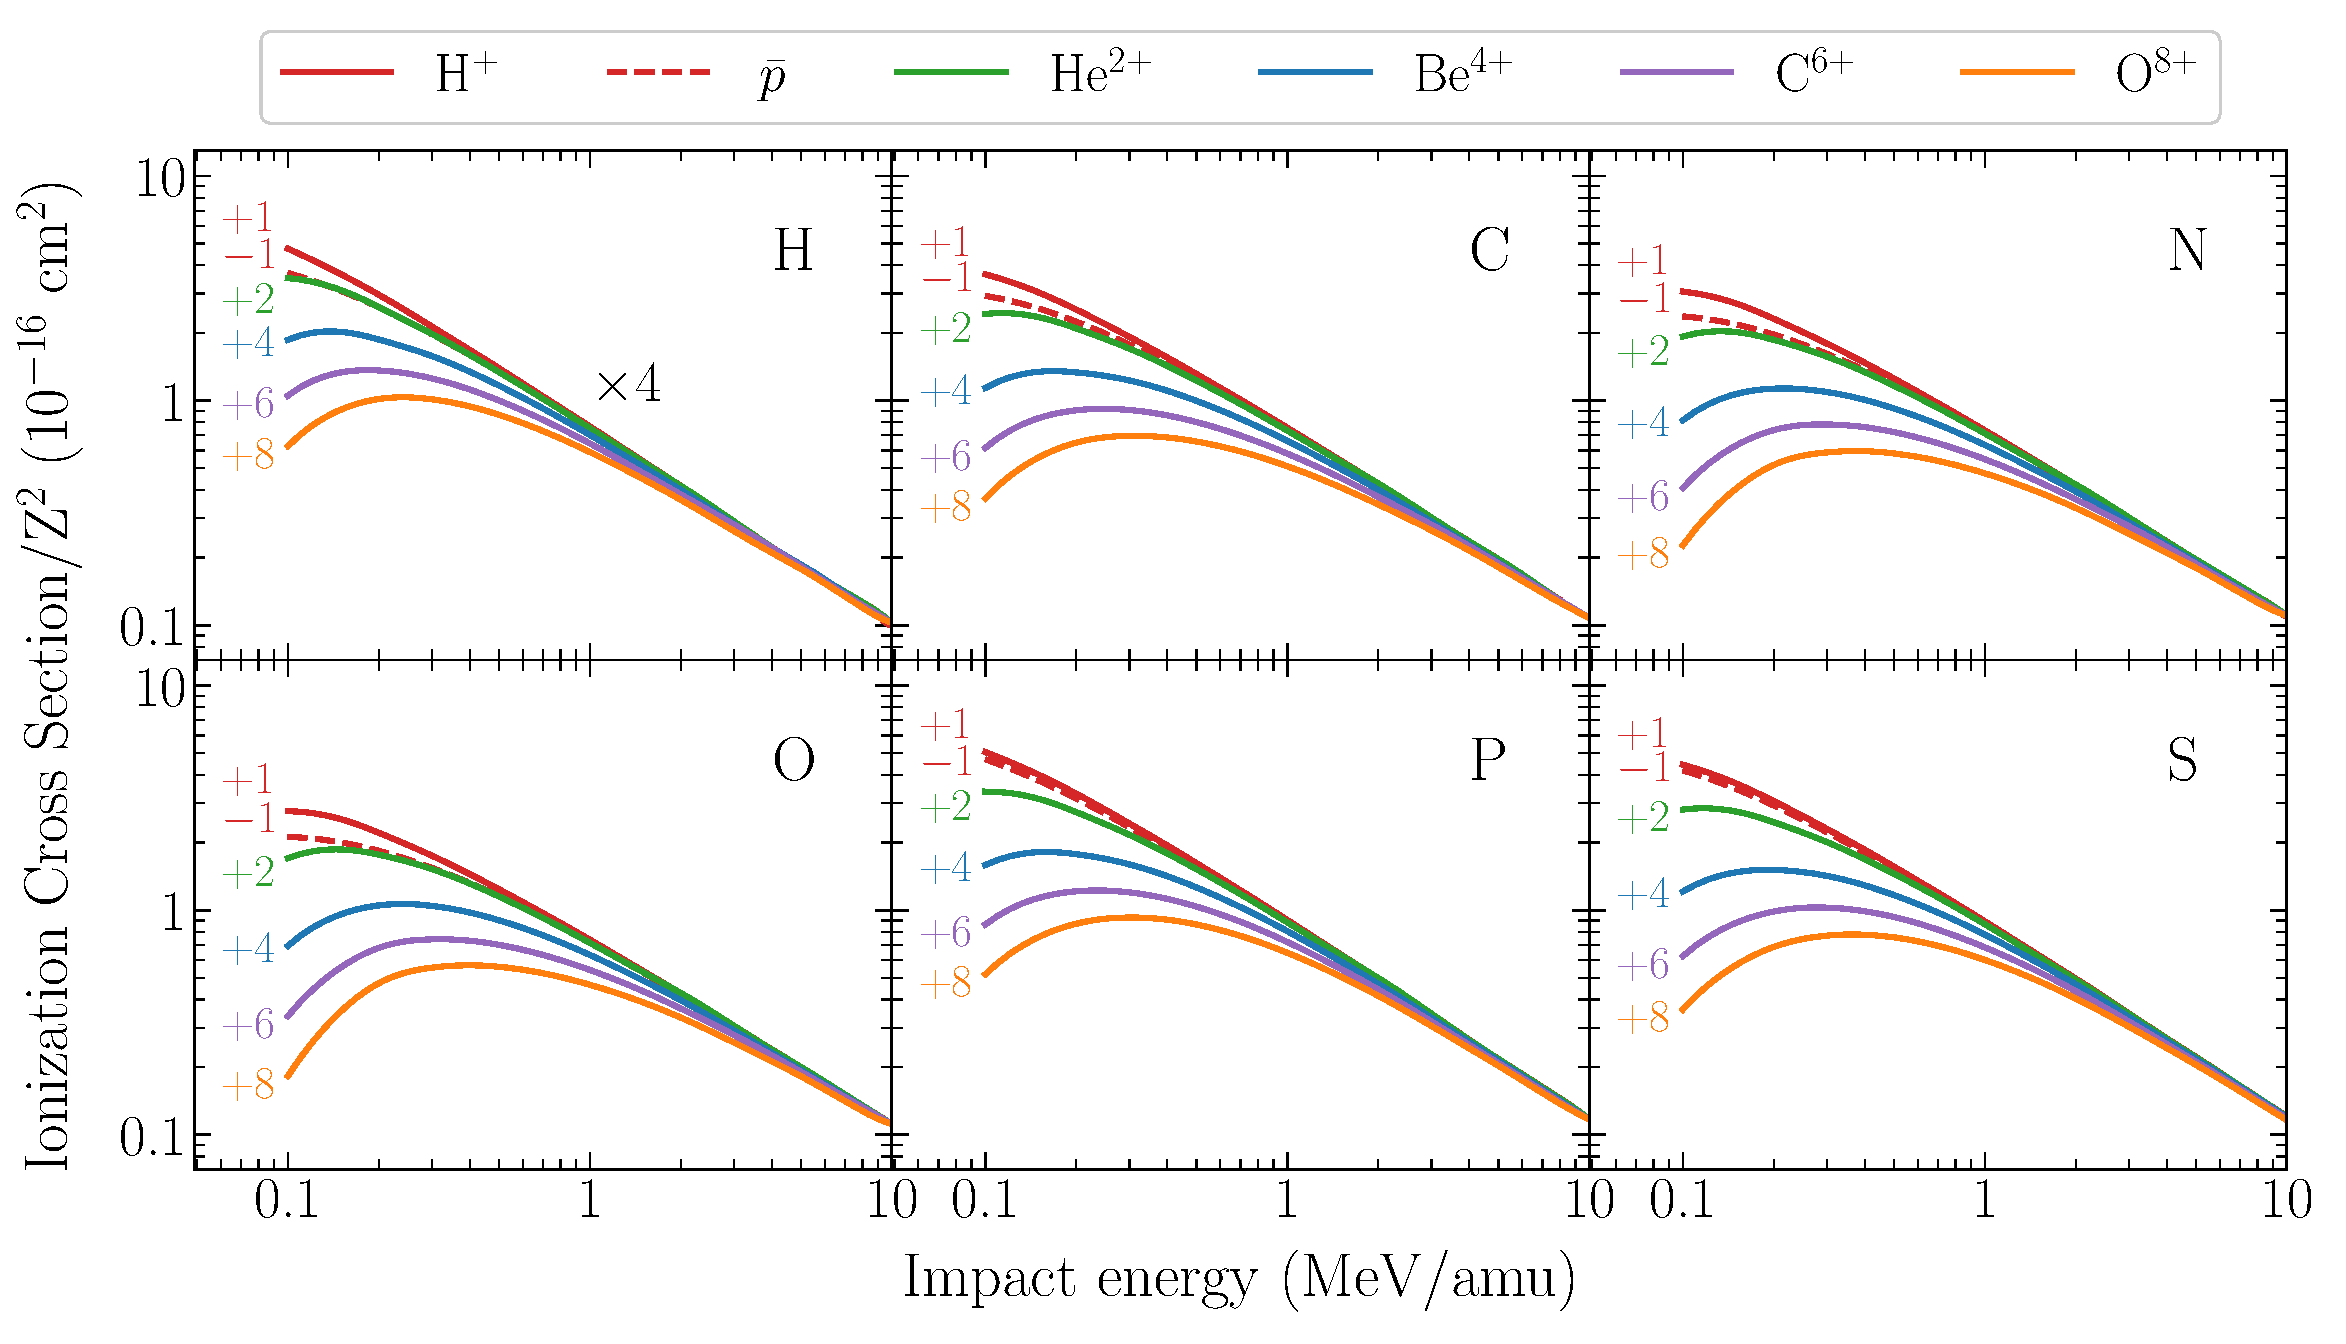
\includegraphics[width=0.9\textwidth]{ionmol/atomicscaling.eps}
\caption[Sección eficaz total de ionización atómica CDW reducida.]
{Sección eficaz total de ionización reducida $\sigma_{\alpha}/Z^2$ 
de cuatro blancos atómicos relevantes. Curvas: cálculos teóricos CDW. 
Símbolos: datos experimentales de H$^+$ en H~\cite{Shah:81}, 
N~\cite{Rudd:85} y O~\cite{Rudd:85}; $e^-$ en 
H~\cite{Shah:87}, C~\cite{Brook:78}, N~\cite{Brook:78} y 
O~\cite{Thompson:95} con conversión de equivelocidad.}
\label{fig:atomscaling}
\end{figure} 

La mayor parte de las moléculas orgánicas contienen átomos de hidrógeno, 
carbono, nitrógeno y oxígeno. Así, los sistemas colisionales que se 
estudian en esta Sección están compuestos por estos cuatro blancos 
atómicos y los proyectiles: antiprotones $\bar{p}$, H$^{+}$, He$^{2+}$, 
Be$^{4+}$, C$^{6+}$, y O$^{8+}$. Particularmente, los estados inicial y 
final de los blancos se obtienen implementando en el 
código~\textsc{radialf}, desarrollado por Salvat y 
colaboradores~\cite{salvat1995}. Las secciones eficaces totales de 
ionización CDW-DIM de los 24 sistemas blanco--proyectil resultantes se 
muestran en la Fig.~\ref{fig:atomscaling}. Los resultados 
correspondientes a cada sistema colisional se presentan en una única 
figura considerando que, en la primera aproximación de Born, la sección 
eficaz de ionización es proporcional al cuadrado de la carga del ion 
incidente, es decir $Z^{2}$. Como puede observarse, este comportamiento 
sólo es válido a altas energías (i.e. $E>5$~MeV/amu). La región 
energética en la cual el método CDW es válido va desde $0.1$ hasta 
10~MeV/amu. Particularmente, para los proyectiles con cargas más altas, 
el valor de energía mínimo donde se espera que la aproximación tenga 
validez aumenta hasta aproximadamente 400~keV. Los valores teóricos CDW 
se comparan con secciones eficaces experimentales disponibles en la 
literatura, tales como la ionización por impacto de H$^+$ en 
H~\cite{Shah:81}, N~\cite{Rudd:85} y O~\cite{Rudd:85}. Para ampliar la 
comparación, se incluyen mediciones de ionización por impacto de 
electrones en H~\cite{Shah:87}, C~\cite{Brook:78}, N~\cite{Brook:78} 
y O~\cite{Thompson:95}, con la correspondiente conversión de energías
para valores superiores a 300~eV. Es esperable que las ionizaciones por 
impacto de H$^+$ y $e^-$ converjan para altas energías del proyectil. 
También se realizaron cálculos similares con la FBA (no se muestran 
aquí), corroborando que ésta provee resultados confiables para valores 
de energía mayores a unos cuantos MeV/amu. Los resultados de ionización 
CDW de cada capa de estos sistemas colisionales se pueden hallar en la 
Ref.~\cite{Miraglia:19}. Detalles sobre el cálculo se encuentran en la
Ref.~\cite{Montanari:17-iongasesnobles}.

A lo largo de este Capítulo se usa el mismo color de línea para indicar 
la carga del proyectil en todas las figuras que muestran resultados de 
ionización por impacto de iones de carga múltiple: discontinua--roja, 
sólida--roja, azul, magenta, oliva y naranja para antiprotones, H$^{+}$, 
He$^{2+}$, Be$^{4+}$, C$^{6+}$, y O$^{8+}$, respectivamente. En el caso 
de los datos experimentales, se usan símbolos de los mismos colores para 
denotar la carga del ion incidente correspondiente y símbolos negros 
para electrones. 

%%%%%%%%%%%%%%%%%%%%%%%%%%%%%%%%%%%%%%%%%%%%%%%%%%%%%%%%%%%%%%%%%%%%%%%%
\subsection{Distribución energética de electrones}
\label{subsec:meanener}
%%%%%%%%%%%%%%%%%%%%%%%%%%%%%%%%%%%%%%%%%%%%%%%%%%%%%%%%%%%%%%%%%%%%%%%%

\begin{figure}
\centering
\includegraphics[width=0.9\textwidth]{ionmol/ener_mean.eps}
\caption[Distribución energética media de electrones emitidos.]
{Distribución energética media de electrones emitidos por la ionización 
debido al impacto de iones de carga múltiple dada por la 
Ec.~(\ref{eq:meanener}). Curvas: cálculos teóricos FBA (punteada) y CDW 
(sólidas y discontinua).}
\label{fig:emittedener}
\end{figure} 

En un medio biológico dado, la ionización directa debido al impacto de 
un ion representa solo una fracción del daño total. Los electrones 
secundarios, así como el retroceso de los iones del blanco, también 
contribuyen sustancialmente al daño total~\cite{Denifl:11}. La sección 
eficaz de ionización diferencial en función de la energía del electrón 
eyectado $E$ de la capa $nl$ del átomo $\alpha$ se puede considerar como 
una función de distribución simple~\cite{Surdutovic:18}. Así, siguiendo 
a Abril y colaboradores~\cite{Abril:15}, se define el valor medio de la 
energía de los electrones ionizados como
$\overline{E}_{\alpha}$, 
\begin{eqnarray}
\overline{E}_{\alpha} &=&\frac{\langle E_{\alpha}\rangle}{\langle
1\rangle}=\frac{1}{\sigma_{\alpha}}\sum\limits_{nl}\int dE\,E
\frac{d\sigma_{\alpha,nl}}{dE}\,,  
\label{eq:meanener} \\
\langle 1\rangle &=&\sigma_{\alpha}=\sum\limits_{nl}\int dE\,
\frac{d\sigma_{\alpha,nl}}{dE}\,. 
\label{eq:normener}
\end{eqnarray}
donde $\Sigma_{nl}$ es la suma de las contribuciones de cada capa del 
elemento $\alpha$.

Las energías medias de los electrones emitidos $\overline{E}_{\alpha}$ 
de H, C, N y O por impacto de $\bar{p}$, H$^{+}$, He$^{2+}$, Be$^{4+}$, 
C$^{6+}$, y O$^{8+}$ se muestran en la Fig.~\ref{fig:emittedener}. 
%A medida que la velocidad de impacto $v$ aumenta, también aumenta 
%$\langle E_{\alpha}\rangle$ y $l_{\max}$, lo que resulta en la inclusión 
%de funciones con muchas oscilaciones en el integrando. Más aún, el 
%integrando de $\langle E_{\alpha}\rangle$ incluye la energía cinética 
%$E$, reduciendo su valor en la región de energías pequeñas e 
%incrementándolo para valores grandes; en consecuencia, las energías de
%ejección medias son más sensibles a los momentos angulares mayores. 
%Independientemente, para $v>10$ a.u., la primera aproximación de Born 
%es válida. 
%
%En la Fig.~\ref{fig:emittedener} se calcula el valor de 
Los valores CDW de $\overline{E}_{\alpha}$ de los electrones emitidos 
están en el rango de energía de 10 a 70 eV para todos los blancos 
atómicos. Estos resultados concuerdan con otros modelos 
teóricos~\cite{Surdutovic:18}. Como se puede observar en la figura, el 
valor de energía media es sensible a la carga del proyectil $Z$, que 
puede duplicar los resultados de protón en la región intermedia, i.e., 
100--400 keV/amu. El efecto observado puede atribuirse a la reducción en 
la emisión de electrones de baja energía por los iones de carga múltiple. 
Este comportamiento no se puede encontrar en la primera aproximación de 
Born, donde la ley de escala $Z^2$ cancela la dependencia con $Z$ de la 
Ec.~(\ref{eq:meanener}). A altas energías, $\overline{E}_{\alpha}$ 
tiende a un valor universal para todos los iones, como puede verse en la 
Fig.~\ref{fig:emittedener}.

%%%%%%%%%%%%%%%%%%%%%%%%%%%%%%%%%%%%%%%%%%%%%%%%%%%%%%%%%%%%%%%%%%%%%%%%
\subsection{Distribución angular de electrones}
\label{subsec:meanang}
%%%%%%%%%%%%%%%%%%%%%%%%%%%%%%%%%%%%%%%%%%%%%%%%%%%%%%%%%%%%%%%%%%%%%%%%

\begin{figure}
\centering
\includegraphics[width=0.9\textwidth]{ionmol/ang_mean.eps}
\caption[Distribución angular media de electrones emitidos.]
{Distribución angular media de electrones emitidos por la ionización 
debido al impacto de iones de carga múltiple dada por 
Ec.~(\ref{eq:meanang}). Curvas: cálculos teóricos FBA (punteada) y CDW 
(sólidas y discontinua).}
\label{fig:emittedang}
\end{figure} 

Como se estableció previamente, la emisión de electrones secundarios 
contribuye al daño total. Por lo tanto, no sólo es esencial conocer la 
distribución de energía de los electrones eyectados, sino también la 
dirección en la que éstos son emitidos. Una vez más, se puede considerar 
que la sección eficaz diferencial de ionización en función del ángulo 
sólido de eyección del electrón $\Omega$ puede expresarse como una 
función de distribución. Así, el ángulo medio de emisión 
$\overline{\theta}_{\alpha}$ se define como 
\begin{eqnarray}
\overline{\theta}_{\alpha}&=&\frac{\langle\theta_{\alpha}\rangle}
{\langle 1\rangle}=\frac{1}{\sigma_{\alpha}}\sum\limits_{nl}
\int d\Omega\,\theta\,\frac{d\sigma_{\alpha,nl}}{d\Omega} 
\label{eq:meanang} \\
\langle 1\rangle &=&\sigma_{\alpha}=\sum\limits_{nl}\int d\Omega\,
\frac{d\sigma_{\alpha,nl}}{d\Omega}\,.
\end{eqnarray}

Los ángulos medios de emisión electrónica $\overline{\theta}_{\alpha}$ 
de los cuatro átomos y seis iones estudiados en esta Sección se muestran 
en la Fig.~\ref{fig:emittedang}. Se puede observar una dependencia 
significativa de $\overline{\theta}_{\alpha}$ con $Z$ para todos los 
sistemas colisionales. Una vez más, este efecto no se observa en la 
implementación de la FBA (línea punteada), ya que es independiente del 
valor de $Z$.

En la emisión de electrones a bajas energías, la dispersión angular es 
casi isotrópica~\cite{Rudd:92}. Un valor típico para el ángulo de 
eyección considerado en la literatura es 
$\overline{\theta}_{\alpha}\sim$~70\textdegree~\cite{Surdutovic:18}, el 
cual resulta bastante certero en el rango de validez de la FBA para 
cualquier blanco. Sin embargo, en el marco de la aproximación de onda 
distorsionada, $\overline{\theta}_{\alpha}$ disminuye sustancialmente 
con $Z$ en la región de energía intermedia. Como se observa en la 
Fig.~\ref{fig:emittedang}, cuanto mayor es la carga $Z$,
$\overline{\theta}$ es menor y el electrón es emitido hacia adelante. 
Por supuesto, este efecto es más notorio en el rango de energías 
intermedias que a altas energías.

Para ilustrar esta fenómeno, consideremos el impacto de C$^{6+}$ con una 
energía de 500~keV sobre oxígeno. En la primera aproximación de Born, la 
teoría predice emisión de electrones con energías medias de $46.7$ eV y 
ángulos medios de 78\textdegree. En cambio, en la aproximación CDW, los 
electrones eyectados tienen energías medias de $62.5$~eV y ángulos de 
emisión iguales a 60\textdegree. Estos resultados sugieren una 
penetración más profunda de los electrones secundarios que la predicha 
por la FBA, con una orientación más cercana a la dirección del ion. La 
correción de la dirección de emisión se puede atribuir al efecto de 
captura del contínuo, incluido en la CDW.

Además, la Fig.~\ref{fig:emittedang} proporciona una descripción 
ilustrativa del comportamiento de los antiprotones: el proyectil repele 
los electrones, siendo $\overline{\theta}_{\alpha}\ge$~90\textdegree a 
bajas energías (emisión hacia atrás). Nótese la diferencia en el ángulo 
de emisión por impacto de protones y antiprotones dada por la CDW 
con respecto a la primera aproximación de Born; este fenómeno constituye 
un efecto Barkas angular~\cite{Sigmud:03}.

%%%%%%%%%%%%%%%%%%%%%%%%%%%%%%%%%%%%%%%%%%%%%%%%%%%%%%%%%%%%%%%%%%%%%%%%
\section{El modelo estequiométrico}
\label{sec:SSM}
%%%%%%%%%%%%%%%%%%%%%%%%%%%%%%%%%%%%%%%%%%%%%%%%%%%%%%%%%%%%%%%%%%%%%%%%

El modelo estequiométrico simple (\acs{ssm}) que se propone para 
predecir secciones eficaces moleculares totales de ionización está 
basado en la aproximación de átomo independiente, también llamada regla 
aditiva de Bragg. Este modelo supone que los átomos que componen una 
molécula $M$ interactúan con el proyectil incidente pero no entre sí. 
Así, si la molécula $M$ está compuesta por $n_{\alpha}$ átomos del 
elemento $\alpha$, el modelo estequiométrico aproxima la sección eficaz 
total de ionización de la molécula $\sigma_M$ como la suma de secciones 
eficaces totales de ionización de los átomos aislados 
$\sigma_{\alpha}$ ponderada por $n_{\alpha}$, 
\begin{equation}
\sigma_{M}=\sum\limits_{\alpha}n_{\alpha}\sigma_{\alpha}\,.  
\label{eq:sumion}
\end{equation}
Los blancos moleculares que se examinan a lo largo de este Capítulo se 
clasifican en tres familias: CH, CHNO, y ADN, como se muestra en la 
Tabla~\ref{tab:families}.

\begin{table}
\begin{center}
\begin{tabularx}{\textwidth}{
>{\centering\arraybackslash}p{0.3\textwidth}
>{\centering\arraybackslash}p{0.3\textwidth}
>{\centering\arraybackslash}p{0.3\textwidth}}
\rowcolor{mydarkgray} 
CH & CHNO & DNA \\
CH$_4$ (metano) & C$_5$H$_5$N (piridina)       & C$_5$H$_5$N$_5$ (adenina) \\
\rowcolor{mygray} 
C$_2$H$_2$ (acetileno) & C$_4$H$_4$N$_2$ (pirimidina)     & C$_4$H$_5$N$_3$O (citosina) \\
C$_2$H$_4$ (eteno)     & C$_2$H$_7$N     (dimetilamina)   & C$_5$H$_5$N$_5$O (guanina) \\
\rowcolor{mygray} 
C$_2$H$_6$ (etano)     & CH$_5$N         (monometilamina) & C$_5$H$_6$N$_2$O$_2$ (timina) \\
C$_6$H$_6$ (benceno)   & C$_4$H$_8$O     (THF)            & C$_4$H$_4$N$_2$O$_2$ (uracilo) \\
\rowcolor{mygray} 
 & & H$_2$O (agua) \\
\end{tabularx}
\caption[Blancos moleculares examinados y clasificados en tres 
familias.]
{Blancos moleculares de interés examinados en el presente trabajo y 
clasificados en tres familias.}
\label{tab:families}
\end{center}
\end{table}

\begin{figure}
\centering
\includegraphics[width=0.9\textwidth]{ionmol/adn1.eps}
\caption[Sección eficaz total de ionización reducida por $Z$ (Parte I).]
{Sección eficaz total de ionización reducida $\sigma_{M}/Z^2$ como 
una función de la energía de impacto del ion. Curvas: cálculos teóricos 
SSM-CDW. Símbolos: datos experimentales de impacto de 
protón~\cite{Iriki:11}, 
C$^{4+}$~\cite{Sens:20}, C$^{6+}$~\cite{Bhattacharjee:19}, y 
e$^-$~\cite{Rahman:16} con conversión de equivelocidad.}
\label{fig:crossDNA_1}
\end{figure} 

En la Fig.~\ref{fig:crossDNA_1} se reportan las secciones eficaces de 
ionización totales reducidas con la carga del ion incidente, 
$\sigma_M/Z^2$, de las nucleobases del ADN --adenina, citosina, guanina 
y timina-- debido al impacto de iones de carga múltiple, que se obtienen 
a partir de la aproximación SSM y el método CDW. Para adenina, los datos 
experimentales disponibles para el impacto de protones~\cite{Iriki:11} 
tienen un excelente acuerdo con las predicciones teóricas. La medición de 
C$^{4+}$~\cite{Sens:20} sobre adenina coincide con el modelo SSM--CDW 
dentro del margen de error. Si bien estos datos son preliminares 
(publicados recientemente en la tesis doctoral de Sens), la comparación 
es alentadora en cuanto a la respuesta del modelo para la ionización por 
proyectiles de carga múltiple. En cambio, los resultados teóricos de 
ionización de adenina debido a C$^{6+}$ discrepan con el valor 
experimental disponible~\cite{Bhattacharjee:19} en un factor dos. Esta 
discrepancia es intrigante ya que la medición se encuentra en el rango 
de altas energías, donde aún la FBA predice muy bien los experimentos.

No se han encontrado en la bibliografía datos experimentales de 
ionización por impacto de iones de carga múltiple para el resto de las 
nucleobases de ADN. En la Fig.~\ref{fig:crossDNA_1} se incluyen 
mediciones de ionización por impacto de electrones~\cite{Rahman:16}, con 
la correspondiente conversión de equivelocidad, para energías incidentes 
superiores a 300~eV. En esta región, las secciones eficaces de 
ionización por impacto de protones y electrones deberían coincidir. Si 
bien las mediciones de ionización por impacto de electrones están por 
encima de las predicciones teóricas presentes para todos los objetivos 
moleculares, los resultados SSM--CDW concuerdan muy bien con otras 
predicciones teóricas de ionización por impacto de 
electrón~\cite{mozejko2003,tan2018}. Más aún, recientes cálculos por 
Zein y colaboradores~\cite{Zein:21} usando el modelo de encuentro 
binario de Bethe sostienen esta tendencia.

\begin{figure}
\centering
\includegraphics[width=0.9\textwidth]{ionmol/adn2.eps}
\caption[Sección eficaz total de ionización reducida por $Z$ 
(Parte II).]
{Sección eficaz total de ionización reducida $\sigma_{M}/Z^2$ como 
una función de la energía de impacto del ion. 
Curvas: cálculos teóricos SSM-CDW. 
Símbolos: datos experimentales de impacto de protón en 
uracilo~\cite{itoh2013}, 
pirimidina~\cite{wolff2014}, THF~\cite{wang2016} y agua~\cite{Luna2007,
Bolorizadeh86,H_Rudd85,toburen80}. Impacto de C$^{4+}$~\cite{Sens:20} y 
C$^{4+}$, C$^{6+}$, O$^{6+}$, F$^{6+}$, O$^{8+}$, y F$^{8+}$ en 
uracilo~\cite{agnihotri2012,agnihotri2013}. Ionización de agua por 
impacto de He$^{2+}$~\cite{Ohsawa05,He_Rudd85,toburen80}, 
C$^{6+}$~\cite{DalCappello:09,Bhattacharjee:17} y 
O$^{8+}$~\cite{Bhattacharjee:16}. 
Impacto de e$^-$~\cite{bug2017,wolf2019,fuss2009} con conversión de 
equivelocidad.}
\label{fig:crossDNA_2}
\end{figure} 

Las secciones eficaces de ionización total reducidas $\sigma_M/Z^2$ 
para uracilo, pirimidina, THF y agua se muestran en la 
Fig.~\ref{fig:crossDNA_2}. En uracilo, las mediciones experimentales de 
ionización por impacto de protones de 
Itoh~\textit{et al.}~\cite{itoh2013} tienen un buen acuerdo con el 
modelo SSM--CDW. Sin embargo, para el mismo blanco, las predicciones 
teóricas difieren en un factor dos de las mediciones experimentales de 
Agnihotri \textit{et al.}~\cite{agnihotri2012,agnihotri2013} para el 
impacto de iones de carga múltiple. No obstante, cabe señalar que los 
resultados teóricos coinciden con los cálculos de Champion, 
Rivarola y colaboradores~\cite{agnihotri2012,champion2012}. Los cálculos 
de Sarkadi~\cite{sarkadi2016}, que emplean el método de trayectorias 
clásicas Monte Carlo, también se encuentran por arriba de estos valores 
experimentales. En la figura también se incluye una reciente medición 
experimental preliminar de Sens \textit{et al.}~\cite{Sens:20} para la 
ionización en uracilo debido al impacto de C$^{4+}$, que coincide con la 
teoría. Si bien los resultados son preliminares, esta discrepancia 
podría indicar algún problema con los valores experimentales de 
Agnihotri y colaboradores. 

Para pirimidina, los cálculos teóricos se comparan con los datos 
experimentales de ionización por impacto de protones de Wolff 
\textit{et al.}~\cite{wolff2014} y por impacto de 
electrones~\cite{bug2017} a altas energías. Las mediciones de electrones 
concuerdan con el modelo SSM--CDW para energías superiores a 500~keV. 
Sin embargo, las secciones eficaces de ionización por impacto de 
protones son significativamente más bajas que la teoría. Una mayor 
cantidad de experimentos se encuentran disponibles para la ionización de 
la molécula de THF por impacto de H$^+$~\cite{wang2016} y de 
e$^-$~\cite{bug2017,wolf2019,fuss2009}. Los resultados que se obtienen 
de la combinación del SSM y las secciones eficaces atómicas CDW muestran 
un buen acuerdo general con esta data.

En el caso de la molécula de agua, los resultados experimentales son más 
abundantes que para el resto de los blancos. Los resultados 
experimentales~\cite{Luna2007,Bolorizadeh86,H_Rudd85,Ohsawa05,He_Rudd85,
toburen80,Bhattacharjee:16} coinciden con las curvas teóricas para 
todos los iones de carga múltiple examinados aquí a excepción de
C$^{6+}$~\cite{DalCappello:09,Bhattacharjee:17}, donde la teoría 
sobrestima la ionización en un factor dos en el rango de altas energías. 
Estas discrepancias podrían suponer fallas en el experimento. 
A diferencia de las nucleobases, pirimidina y THF, la estequiometría del 
agua es más simple; sin embargo, observamos que nuestro modelo responde 
bien incluso para predecir la ionización de moléculas pequeñas debido a 
la incidencia de iones pesados, tal como es el caso de O$^{6+}$.

%%%%%%%%%%%%%%%%%%%%%%%%%%%%%%%%%%%%%%%%%%%%%%%%%%%%%%%%%%%%%%%%%%%%%%%%
\section{Reglas de escala}
\label{sec:scaling}

%%%%%%%%%%%%%%%%%%%%%%%%%%%%%%%%%%%%%%%%%%%%%%%%%%%%%%%%%%%%%%%%%%%%%%%%
\subsection{Escala con electrones activos del blanco}
\label{subsec:ne_scaling}

%%%%%%%%%%%%%%%%%%%%%%%%%%%%%%%%%%%%%%%%%%%%%%%%%%%%%%%%%%%%%%%%%%%%%%%%
\subsubsection*{Regla de Toburen}
\label{subsec:toburen}
%%%%%%%%%%%%%%%%%%%%%%%%%%%%%%%%%%%%%%%%%%%%%%%%%%%%%%%%%%%%%%%%%%%%%%%%

Toburen y colaboradores~\cite{Toburen:75,Toburen:76} propusieron el 
primer modelo fenomenológico completo y simple para la eyección de 
electrones de moléculas complejas. Los autores encontraron conveniente 
escalar la sección eficaz de ionización experimental en términos del 
número de electrones ligados débilmente, también llamados activos, 
$n_e$. En general, este valor está dado por la cantidad de electrones 
en la capa de valencia. Así, por ejemplo, para C, N y O, este número es 
igual al total de electrones del átomo menos la capa K. 

Siguiendo a Toburen \textit{et al.}, se define la sección eficaz de 
ionización reducida por el número de electrones débilmente ligado 
$\sigma_e$ para la molécula $M$ como
\begin{equation}
\sigma_e=\frac{\sigma_M}{n_e}\,, 
\label{eq:cross-ne} 
\end{equation}
donde $n_e=\sum_{\alpha}n_{\alpha}\nu_{\alpha}$ es el número total de 
electrones activos en el proceso colisional, y $\nu_{\alpha}$ es el 
número de electrones débilmente ligado en cada átomo $\alpha$. Los 
números de Toburen de los blancos atómicos considerados en este trabajo 
están dados por 
\begin{equation}
\nu_{\alpha}^T=\left\{ 
\begin{array}{ll}
1, & \text{para H,} \\
4, & \text{para C,} \\ 
5, & \text{para N,} \\ 
6, & \text{para O}\,.
\end{array}\right.
\label{eq:neToburen} 
\end{equation} 

La regla de Toburen se puede enunciar diciendo que $\sigma_{e}$ es un 
parámetro universal, que depende únicamente de la velocidad y naturaleza
del ion incidente. Esta regla es aplicable en la región de $0.25$ a 
5~MeV/amu. A muy altas energías, la probabilidad de ionizar electrones 
de la capa K es relevante y el número total de electrones activos será 
diferente. Una dependencia similar con el número de electrones 
débilmente ligados fue hallada por Itoh y colaboradores~\cite{itoh2013} 
para el impacto de protones sobre uracilo y adenina.

Siguiendo la ley de escala de Toburen, las secciones eficaces CDW son 
divididas con el número de electrones activos de Toburen, 
$\sigma_{e}^T$, para los blancos moleculares dados en la 
Tabla~\ref{tab:families}. Los resultados de esta implementación se 
muestran en la Fig.~\ref{fig:newscaling}(a) en función de la energía de 
impacto para diferentes proyectiles de carga múltiple. Aunque la escala 
de Toburen se mantiene para altas energías, su desempeño no es muy 
satisfactorio: como se puede observar en la figura, la banda universal 
es bastante ancha.

\begin{figure}[t]
\centering
\includegraphics[width=0.9\textwidth]{ionmol/CDWscaling.eps}
\caption[Sección eficaz de ionización molecular reducida por $n_e$.]
{Sección eficaz de ionización molecular reducida con el número de 
electrones débilmente ligados usando 
(a)~los números de Toburen $\nu_{\alpha}^T$, y 
(b) los números CDW $\nu_{\alpha}^{\text{CDW}}$ propuestos para las 
moléculas enlistadas en la Tabla~\ref{tab:families}. 
Símbolos: datos experimentales de las Figs.~\ref{fig:crossDNA_1} y 
\ref{fig:crossDNA_2}.}
\label{fig:newscaling}
\end{figure}

%%%%%%%%%%%%%%%%%%%%%%%%%%%%%%%%%%%%%%%%%%%%%%%%%%%%%%%%%%%%%%%%%%%%%%%%
\subsubsection*{Números CDW}
\label{subsec:CDW}
%%%%%%%%%%%%%%%%%%%%%%%%%%%%%%%%%%%%%%%%%%%%%%%%%%%%%%%%%%%%%%%%%%%%%%%%

La respuesta del modelo teórico SSM--CDW a la regla de escala de Toburen 
se puede entender inspeccionando la Fig.~\ref{fig:neCDW}. La figura 
muestra las secciones eficaces de ionización CDW de los átomos H, C, N y 
O debido al impacto de H$^+$ reducidas por el número de electrones 
activos de cada átomo. La Fig.~\ref{fig:neCDW}(a) muestra los resultados 
CDW divididos por los números de Toburen dados por la 
Ec.~(\ref{eq:neToburen}). La regla de Toburen no se cumple de manera 
apropiada por los cálculos CDW: para un valor de energía dado, los 
valores teóricos de ionización reducidos 
$\sigma_{\alpha}/\nu_{\alpha}^T$ de cada blanco atómico no son 
constantes. Por otro lado, considerando los valores teóricos de 
ionización de oxígeno dados en la Fig.~\ref{fig:atomscaling}, se observa 
que éstos son muy similares a las secciones eficaces del carbono. Estas 
predicciones parecen sugerir que el número de electrones activos en el 
átomo de O es cuatro en lugar de seis. De la misma manera, el número de 
electrones activos para N, que se obtienen a partir de los resultados 
teóricos CDW, son diferentes de los dados por la 
Ec.~(\ref{eq:neToburen}). La Fig.~\ref{fig:neCDW}(b) muestra la 
respuesta de los cálculos atómicos a estos nuevos valores.

\begin{figure}[t]
\centering
\includegraphics[width=0.9\textwidth]{ionmol/neCDW.eps}
\caption[Sección eficaz de ionización atómica reducida por $n_e$.]
{Sección eficaz de ionización atómica por impacto de H$^+$ reducida con 
el número de electrones débilmente ligados usando 
(a)~los números de Toburen $\nu_{\alpha}^T$, y 
(b) los números CDW $\nu_{\alpha}^{\text{CDW}}$.}
\label{fig:neCDW}
\end{figure}

A partir del estudio sistemático de las predicciones CDW para los 
sistemas proyectil--átomo, se propone una optimización a la regla de 
Toburen. El número total de electrones activos de la molécula $M$ en la 
Ec.~(\ref{eq:cross-ne}) está ahora dado por 
\begin{equation}
n_e'=\sum_{\alpha}n_{\alpha}\nu_{\alpha}^{\text{CDW}}\,,
\label{eq:neprima}
\end{equation}
donde $\nu_{\alpha}^{\text{CDW}}$ son los números de electrones activos 
por átomo, que se obtienen de ajustar las secciones eficaces de 
ionización CDW atómicas. Los números CDW están dados por
\begin{equation}
\nu_{\alpha }^{\text{CDW}} \sim\left\{ 
\begin{array}{ll}
1, & \text{para H,} \\
4, & \text{para C, N, y O}\,. \\ 
\end{array}
\right. 
\label{eq:neCDW}
\end{equation}

A partir de la Ec.~(\ref{eq:neCDW}), se definen nuevos números de 
electrones activos $n_e'$ para las moléculas consideradas hasta ahora.  
La Tabla~\ref{tab:ne_molecules} muestra los valores optimizados $n_e'$ y 
los números de Toburen $n_e$ para una gran variedad de sistemas 
moleculares. Los resultados SSM--CDW son diferentes a los propuestos por 
Toburen, los cuales se han utilizado por otros autores~\cite{itoh2013}. 
La diferencia principal se encuentra en los números de electrones 
activos del oxígeno, y por lo tanto en las moléculas que lo incluyen. 
Las secciones eficaces moleculares divididas por $n_e'$ se muestran en 
la Fig.~\ref{fig:newscaling}(b). Los datos experimentales para la 
ionización de adenina~\cite{Iriki:11,Sens:20,Bhattacharjee:19}, 
uracilo~\cite{itoh2013,Sens:20}, pirimidina~\cite{wolff2014}, 
THF~\cite{wang2016} y agua~\cite{Luna2007,Bolorizadeh86,H_Rudd85,
toburen80,Ohsawa05,He_Rudd85,DalCappello:09,Bhattacharjee:17,
Bhattacharjee:16} por impacto de iones de carga múltiple que se muestran 
en la Fig.~\ref{fig:newscaling}(b) validan nuestra optimización. También 
incluimos mediciones de ionización por impacto de electrones con 
conversión de equivelocidad en pirimidina~\cite{bug2017} y 
THF~\cite{bug2017,wolf2019,fuss2009}. 

\begin{table}[t]
\begin{center}
\begin{tabularx}{\textwidth}{
>{\centering\arraybackslash}p{0.13\textwidth}
>{\centering\arraybackslash}p{0.17\textwidth}
>{\centering\arraybackslash}p{0.04\textwidth}
>{\centering\arraybackslash}p{0.04\textwidth}
>{\centering\arraybackslash}p{0.13\textwidth}
>{\centering\arraybackslash}p{0.17\textwidth}
>{\centering\arraybackslash}p{0.04\textwidth}
>{\centering\arraybackslash}p{0.04\textwidth}}
\rowcolor{mydarkgray} 
Molécula        & Nombre      & $n_e$ & $n_e'$ & 
Molécula        & Nombre      & $n_e$ & $n_e'$ \\
H$_2$           & Dihidrógeno & 2      & 2     & 
C$_4$H$_4$N$_2$ & Pirimidina  & 30     & 28    \\
\rowcolor{mygray} 
H$_2$O          & Agua        & 8      & 6     & 
C$_6$H$_6$      & Etano       & 30     & 30    \\
NH$_3$          & Amoníaco    & 8      & 7     & 
C$_4$H$_4$N$_2$O$_2$ & Uracilo & 40    & 36    \\
\rowcolor{mygray} 
CH$_4$          & Metano      & 8      & 8     & 
C$_4$H$_5$N$_3$O & Citosina   & 42     & 37    \\
CH$_5$N         & Metilamina  & 14     & 13    & 
C$_5$H$_6$N$_2$O$_2$ & Timina & 48     & 42    \\
\rowcolor{mygray} 
C$_2$H$_7$N     & Etilamina   & 20     & 19    & 
C$_5$H$_5$N$_5$ & Adenina     & 50     & 45    \\
C$_4$H$_8$O     & THF         & 30     & 28    & 
C$_5$H$_5$N$_5$O & Guanina    & 56     & 49    \\
\end{tabularx}
\caption[Números de electrones activos moleculares de Toburen y CDW.]
{Número de electrones débilmente ligados según Toburen $n_e$ y 
optimización CDW~$n_e'$ para algunos blancos moleculares de interés 
biológico.}
\label{tab:ne_molecules}
\end{center}
\end{table}

\begin{figure}[t]
\centering
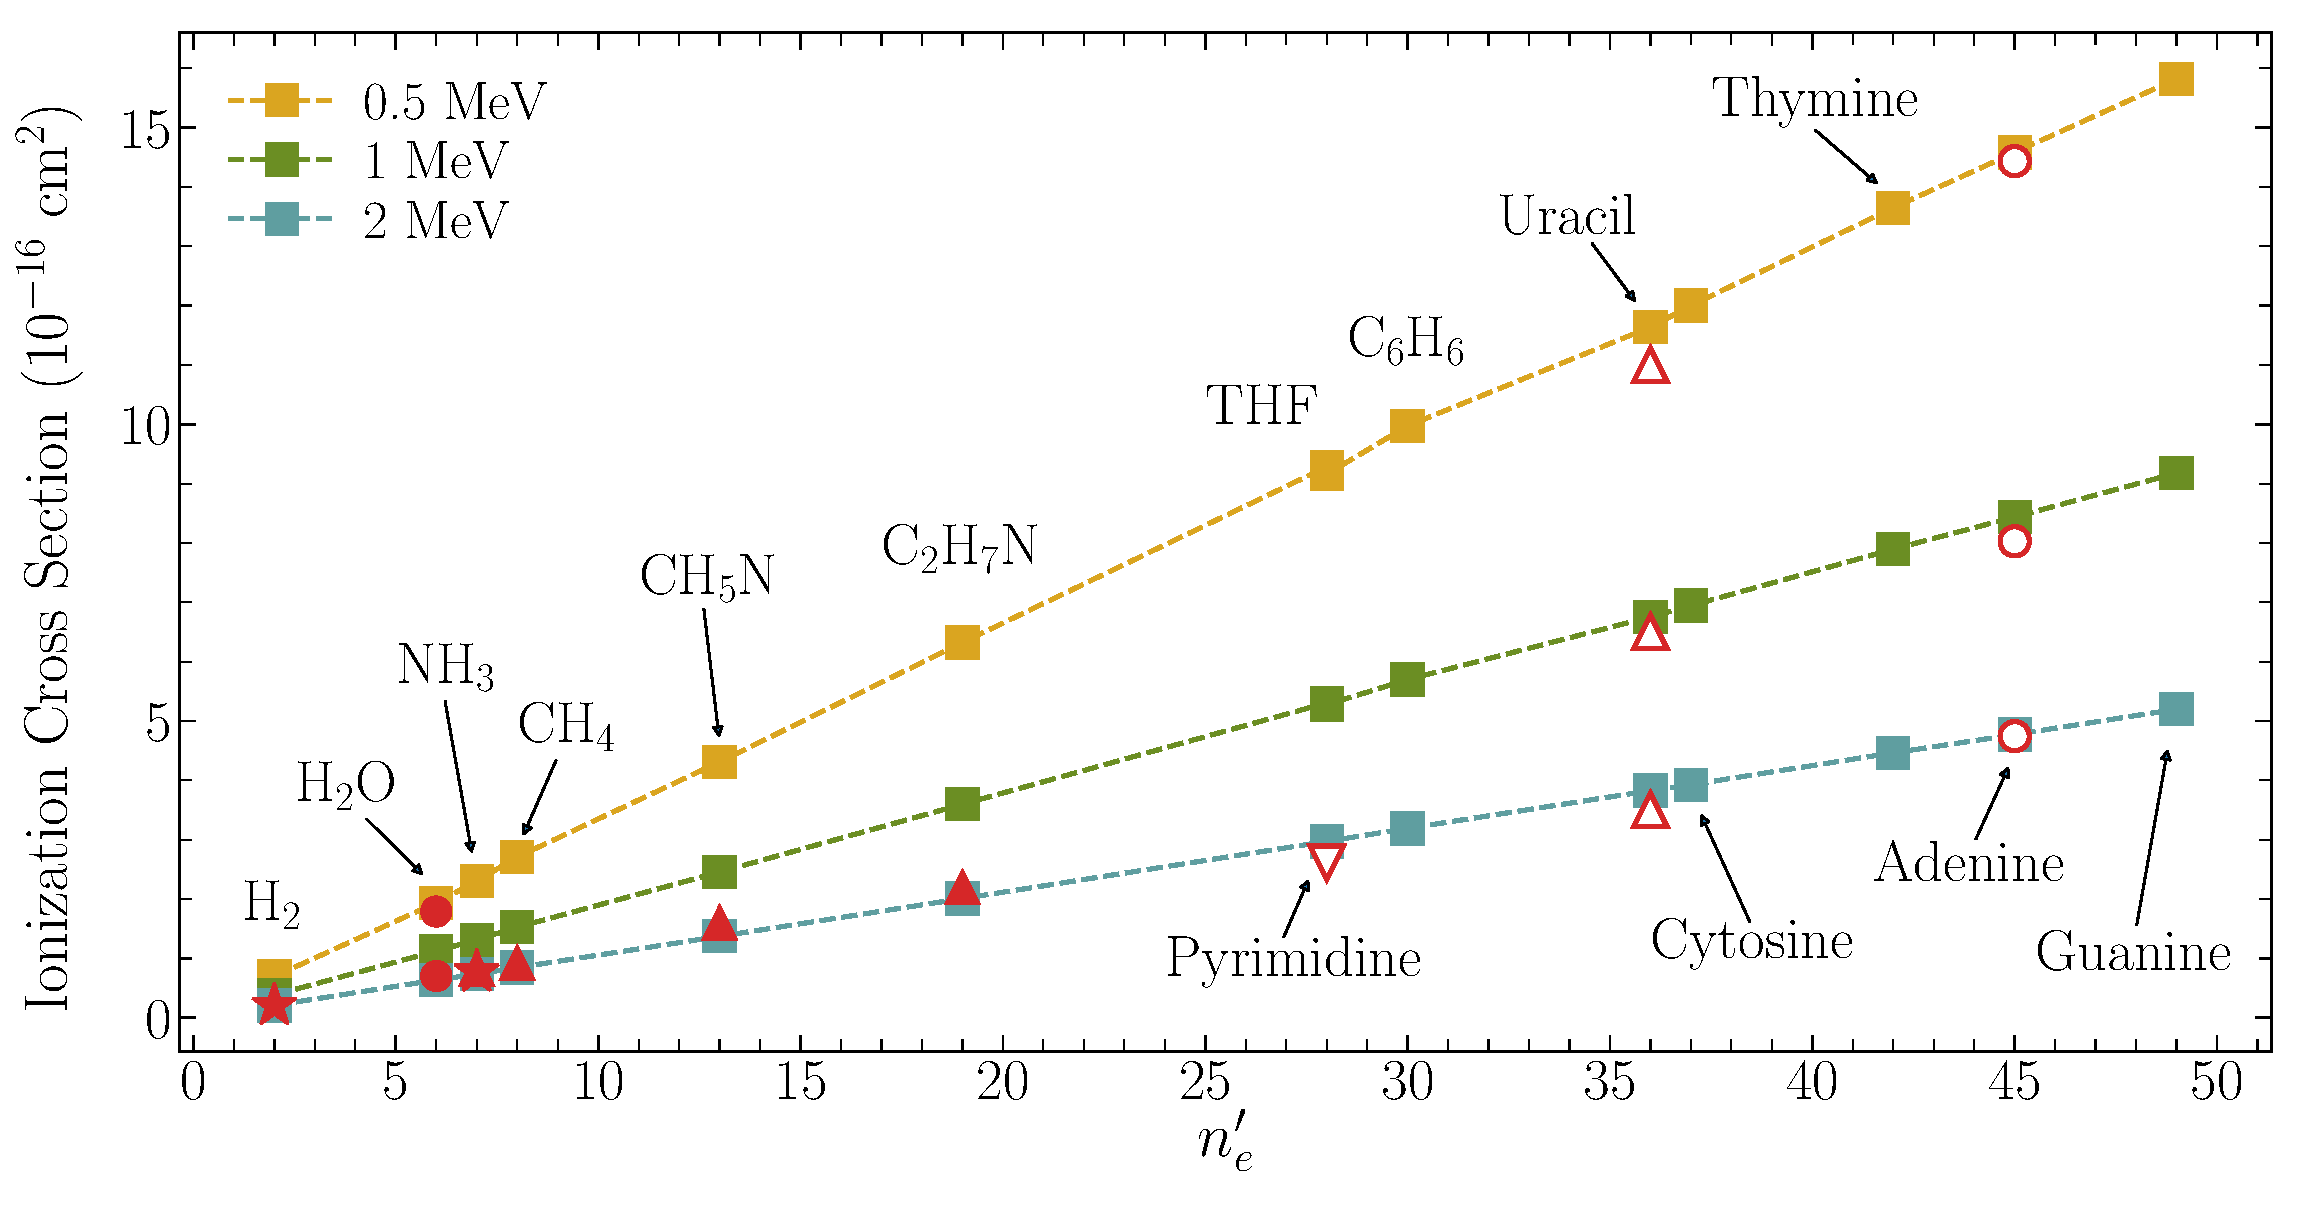
\includegraphics[width=0.9\textwidth]{ionmol/scale_ne.eps}
\caption[Ionización por impacto de protón en términos de $n_e'$.]
{Sección eficaz de ionización por impacto de protón a $0.5$, 1, y 2~MeV 
en términos del número de electrones activos dado por la 
Tabla~\ref{tab:ne_molecules}. Curvas: cálculos teóricos SSM-CDW. 
Símbolos: datos experimentales de 
\mbox{\Large$\circ$}~adenina~\cite{Iriki:11}, 
$\triangle$ uracilo~\cite{itoh2013}, 
$\bigtriangledown$ pirimidina~\cite{wolff2014}, 
$\blacktriangle$ C$_2$H$_7$N, CH$_5$N, metano y amoníaco~\cite{Lynch:76},
\mbox{\scriptsize$\bigstar$} amoníaco y H$_2$~\cite{Rudd:85}, y 
\mbox{\Large$\bullet$} agua~\cite{Luna2007}.}
\label{fig:recta}
\end{figure}

La escala definida por los números CDW se puede examinar de forma 
alternativa dibujando las secciones eficaces de ionización de las 
moléculas en función de $n_e'$ para ciertos valores de energía. Los 
resultados SSM-CDW reducidos se muestran en la Fig.~\ref{fig:recta} para 
energías de impacto de $0.5$, 1 y 2~MeV. Como puede observarse, las 
secciones eficaces de ionización calculadas para todas las moléculas 
muestran una dependencia lineal con el número de electrones CDW $n_e'$ 
de la Tabla~\ref{tab:ne_molecules}. Se obtienen resultados similares 
incluso para $E=10$~MeV (no los incluimos por claridad en la figura). La 
comparación con los datos experimentales disponibles muestra una buena 
concordancia general, desde moléculas pequeñas~\cite{Lynch:76,Rudd:85,
Luna2007}, tales como H$_2$, CH$_4$ y NH$_3$, hasta las más 
complejas~\cite{Iriki:11,itoh2013,wolff2014}, como la adenina. Para los 
datos de ionización por impacto de electrón, los valores experimentales 
se interpolaron entre vecinos cercanos. 

Será interesante verificar la regla de escala optimizada que se presenta
aquí con experimentos futuros, principalmente para estados de carga de 
proyectiles más altos. Por lo pronto, incluso los recientes cálculos 
preliminares de Vera \textit{et al.}~\cite{deVera:20} para la ionización 
de biomateriales por impacto de electrones tienen una respuesta 
satisfactoria a esta regla de escala en todo el rango de energías.
Por otro lado, en el reciente trabajo de 
L\"udde~\textit{et al.}~\cite{Ludde:19} sobre la ionización de 
moléculas biológicas por impacto de protones, los autores hallaron los 
mismos valores de escala para N y O. El acuerdo con este modelo 
independiente refuerza la ley de escala dada por los números de 
electrones activos CDW.

%%%%%%%%%%%%%%%%%%%%%%%%%%%%%%%%%%%%%%%%%%%%%%%%%%%%%%%%%%%%%%%%%%%%%%%%
\subsection{Escala con la carga del ion}
\label{sec:zscaling}
%%%%%%%%%%%%%%%%%%%%%%%%%%%%%%%%%%%%%%%%%%%%%%%%%%%%%%%%%%%%%%%%%%%%%%%%

A energías de impacto intermedias, la regla $Z^2$ no es válida y se 
pueden considerar otras escalas. En la literatura, se encuentran dos 
tipos de leyes de escala con la carga $Z$ del ion incidente aplicables 
en este rango de energías de impacto. La regla sugerida por Janev y 
Presnyakov~\cite{Janev:80} considera $\sigma/Z$ en función de $E/Z$ como 
la forma reducida \textit{natural} de la sección eficaz de ionización 
$\sigma$ y la energía de ion incidente $E$. Más recientemente, 
Montenegro y colaboradores~\cite{Dubois:13,Montenegro:13} sugieren una 
expresión alternativa, la cual toma en cuenta que la sección eficaz es 
una función de $Z^2/E$ a altas energías. La escala propuesta, dada por
\begin{equation}
 \sigma/Z^{\alpha}=f(E/Z^{2-\alpha}),
\label{eq:Montenegro}
\end{equation}
mantiene la relación $Z^2/E$ para cualquier valor del parámetro 
$\alpha$. Los autores proponen el valor $\alpha=4/3$ para la ionización 
de He y H$_2$ debido al impacto de diversos iones 
cargados~\cite{Dubois:13}. 

Siguiendo el trabajo de Montenegro y colaboradores, el 
parámetro~$\alpha$ es optimizado de manera tal que los resultados 
obtenidos por la combinación del método CDW y SSM para los sistemas 
colisionales moleculares estudiados aquí convergan en el mayor rango de 
energías posible (de intermedias a altas). El resultado de dicha 
optimización está dado por $\alpha=1.2$. La validez de este valor 
particular es evidente en las Figs.~\ref{fig:zreduced-adn1} (adenina, 
citosina, timina y guanina) y~\ref{fig:zreduced-adn2} (uracilo, 
pirimidina, THF y agua), donde --para cada blanco-- las curvas SSM--CDW 
correspondientes a los diferentes iones se superponen. Es notable como 
el escaleo de los resultados teóricos SSM-CDW es válido para energías de 
impacto incluso por encima del máximo de las secciones eficaces, que 
corresponden a rangos de energías incidentes desde 50 keV para H$^+$ 
hasta 250 keV/amu para O$^{+8}$.

\begin{figure}
\centering
\includegraphics[width=0.9\textwidth]{ionmol/adn1_zscale.eps}
\caption[Sección eficaz de ionización reducida por $Z$ y $\alpha$ 
(Parte I).]
{Sección eficaz de ionización reducida $\sigma/Z^{\alpha}$ como función
de la energía incidente del ion $E/Z^{2-\alpha}$ con $\alpha=1.2$. 
Curvas: resultados teóricos CDW-SSM. 
Símbolos: datos experimentales de la Fig.~\ref{fig:crossDNA_1}.}
\label{fig:zreduced-adn1}
\end{figure} 

\begin{figure}
\centering
\includegraphics[width=0.9\textwidth]{ionmol/adn2_zscale.eps}
\caption[Sección eficaz de ionización reducida por $Z$ y $\alpha$ 
(Parte II).]
{Sección eficaz de ionización reducida $\sigma/Z^{\alpha}$ como función
de la energía incidente del ion $E/Z^{2-\alpha}$ con $\alpha=1.2$. 
Curvas: resultados teóricos CDW-SSM. 
Símbolos: datos experimentales de la Fig.~\ref{fig:crossDNA_2}.}
\label{fig:zreduced-adn2}
\end{figure} 

Los datos experimentales disponibles para los sistemas ion-blanco bajo 
estudio~\cite{Iriki:11,Sens:20,Bhattacharjee:19,itoh2013,wolff2014,
wang2016,agnihotri2012,agnihotri2013,Luna2007,Bolorizadeh86,H_Rudd85,
He_Rudd85,toburen80,Ohsawa05,Bhattacharjee:17,DalCappello:09,
Bhattacharjee:16} también son examinados con la regla de escala 
$Z^\alpha$. Al igual que en las figuras previas, en el caso de los 
blancos con pocos o ningún dato experimental se incluyen las secciones 
eficaces experimentales de ionización por impacto de 
electrón~\cite{Rahman:16,bug2017,wolf2019,fuss2009} a grandes 
velocidades con la conversión correspondiente. Como se observa, la 
mayoría de los datos experimentales en la Figs.~\ref{fig:zreduced-adn1} 
y \ref{fig:zreduced-adn2} confirma el escaleo sugerido aquí, incluso 
para O$^{+8}$ en agua~\cite{Bhattacharjee:16}. 

%%%%%%%%%%%%%%%%%%%%%%%%%%%%%%%%%%%%%%%%%%%%%%%%%%%%%%%%%%%%%%%%%%%%%%%%
\subsection{Escala con electrones activos y carga del ion}
\label{sec:nez_scaling}
%%%%%%%%%%%%%%%%%%%%%%%%%%%%%%%%%%%%%%%%%%%%%%%%%%%%%%%%%%%%%%%%%%%%%%%%

Considerando la reducción con la carga del ion incidente $Z^\alpha$ y  
el número de electrones activos del blanco $n_e'$, se introduce la 
sección eficaz de ionización molecular independiente $\tilde{\sigma}$, 
que se expresa como función de $\tilde{E}=E/Z^{2-\alpha}$, y está dada 
por 
\begin{equation}
\tilde{\sigma}\left(\tilde{E}\right)=\frac{\sigma_e}{Z^{\alpha}}
=\frac{\sigma_M}{n_e'\,Z^{\alpha}}\,,
\label{eq:u-scaling}
\end{equation}
donde $\sigma_M$ es la sección eficaz de ionización de un blanco 
molecular, $\alpha=1.2$ es el parámetro de ajuste y $n_e'$ es el número 
de electrones activos de la molécula dado las Ecs.~(\ref{eq:neprima}) y 
(\ref{eq:neCDW}). La Fig.~\ref{fig:zalpha} muestra los valores teóricos 
y experimentales de $\tilde{\sigma}$ para todos los sistemas moleculares 
de la Tabla~\ref{tab:families}. Como se observa, la regla de escala 
combinada funciona muy bien y es independiente tanto de la naturaleza 
del ion incidente como de la complejidad del blanco molecular. Los 
resultados teóricos SSM--CDW se ubican en una banda estrecha válida para 
cualquier ion incidente (reducida con $Z^\alpha$) en cualquier molécula 
(contraída con el número de electrones activos $n_e'$) con una 
dispersión de aproximadamente $\pm 20\%$. A partir de los resultados 
teóricos SSM--CDW, se define una expresión paramétrica
\begin{equation}
\Sigma(E)= \frac{a_0}{E} \ln \left( a_1 E - a_2 \right)\,,
\end{equation}
donde $a_0=0.04541$, $a_1=105.3$ y $a_2=2.314$, que ajusta los valores 
teóricos y experimentales con una dispersión del $\pm 35\%$. La curva 
paramétrica se muestra en la figura con una línea discontinua, mientras 
que la dispersión se ilustra con un área gris. Nótese que no hemos 
incluido en esta figura los resultados para uracilo de las 
Refs.~\cite{agnihotri2012,agnihotri2013}. 

\begin{figure}[t]
\centering
\includegraphics[width=0.9\textwidth]{ionmol/Zne_scaling.eps}
\caption[Sección eficaz de ionización reducida por $Z$ y $n_e$.]
{Sección eficaz de ionización reducida con la carga $Z$ del ion 
incidente y con el número de electrones activo $n_e$ del blanco 
molecular, dado por la Ec.~(\ref{eq:u-scaling}) con $\alpha=1.2$. 
Curvas: cálculos teóricos CDW-SSM (líneas sólidas) y ajuste paramétrico 
(línea discontinua). Símbolos: datos experimentales de las 
Figs.~\ref{fig:crossDNA_1} y \ref{fig:crossDNA_2}.}
\label{fig:zalpha}
\end{figure} 

Bajo la hipótesis de que la regla de escala independiente propuesta aquí 
es válida para cualquier combinación ion--molécula, se aplica la regla 
universal a un conjunto de valores experimentales no considerados en la
formulación de nuestro modelo. En la Fig.~\ref{fig:zalpha} se muestran 
las mediciones reducidas de Rudd~\textit{et al.}~\cite{Rudd:85,Rudd:83} 
para H$^{+}$ y He$^{+2}$ en N$_2$, O$_2$, CH$_4$, CO y CO$_2$, y los 
recientes experimentos de Luna~\textit{et al.} \cite{Luna2019} de 
H$^{+}$ en CH$_4$. Los valores experimentales que se incluyen en la 
figura están dentro de la incertidumbre provisto por la regla general.

El buen acuerdo entre los resultados previstos por la escala 
independiente y los datos experimentales disponibles que se muestran en 
la Fig.~\ref{fig:zalpha} resume los principales resultados de esta 
investigación. El modelo muestra ser eficaz no solo para predecir la 
ionización de los sistemas ion--blanco estudiados aquí sino también 
muestra potencial para reproducir una gran variedad de sistemas 
colisionales. Aunque los resultados teóricos SSM--CDW son válidos para 
energías mayores a las del máximo de la sección eficaz de ionización, 
se puede observar en la Fig.~\ref{fig:zalpha} que los datos 
experimentales siguen la regla de escala aún para valores de energía 
incidente menores. Se espera que mediciones experimentales para otros 
iones y moléculas refuercen el modelo teórico y la regla independiente 
propuestos.

%%%%%%%%%%%%%%%%%%%%%%%%%%%%%%%%%%%%%%%%%%%%%%%%%%%%%%%%%%%%%%%%%%%%%%%%
\section{Estructura molecular de los blancos}
\label{sec:molcalculations}
%%%%%%%%%%%%%%%%%%%%%%%%%%%%%%%%%%%%%%%%%%%%%%%%%%%%%%%%%%%%%%%%%%%%%%%%

Finalmente, para estudiar el rango de validez del SSM, hemos calculado 
la estructura molecular de las cinco nucleobases --adenina, citosina, 
guanina, timina y uracilo-- empleando el código {\sc gamess}. Los 
cálculos de energía se realizaron implementando el método restringido de 
Hartree--Fock con optimización de geometría y el conjunto de bases 
gaussianas 3-21G. 

\begin{figure}[t]
\centering
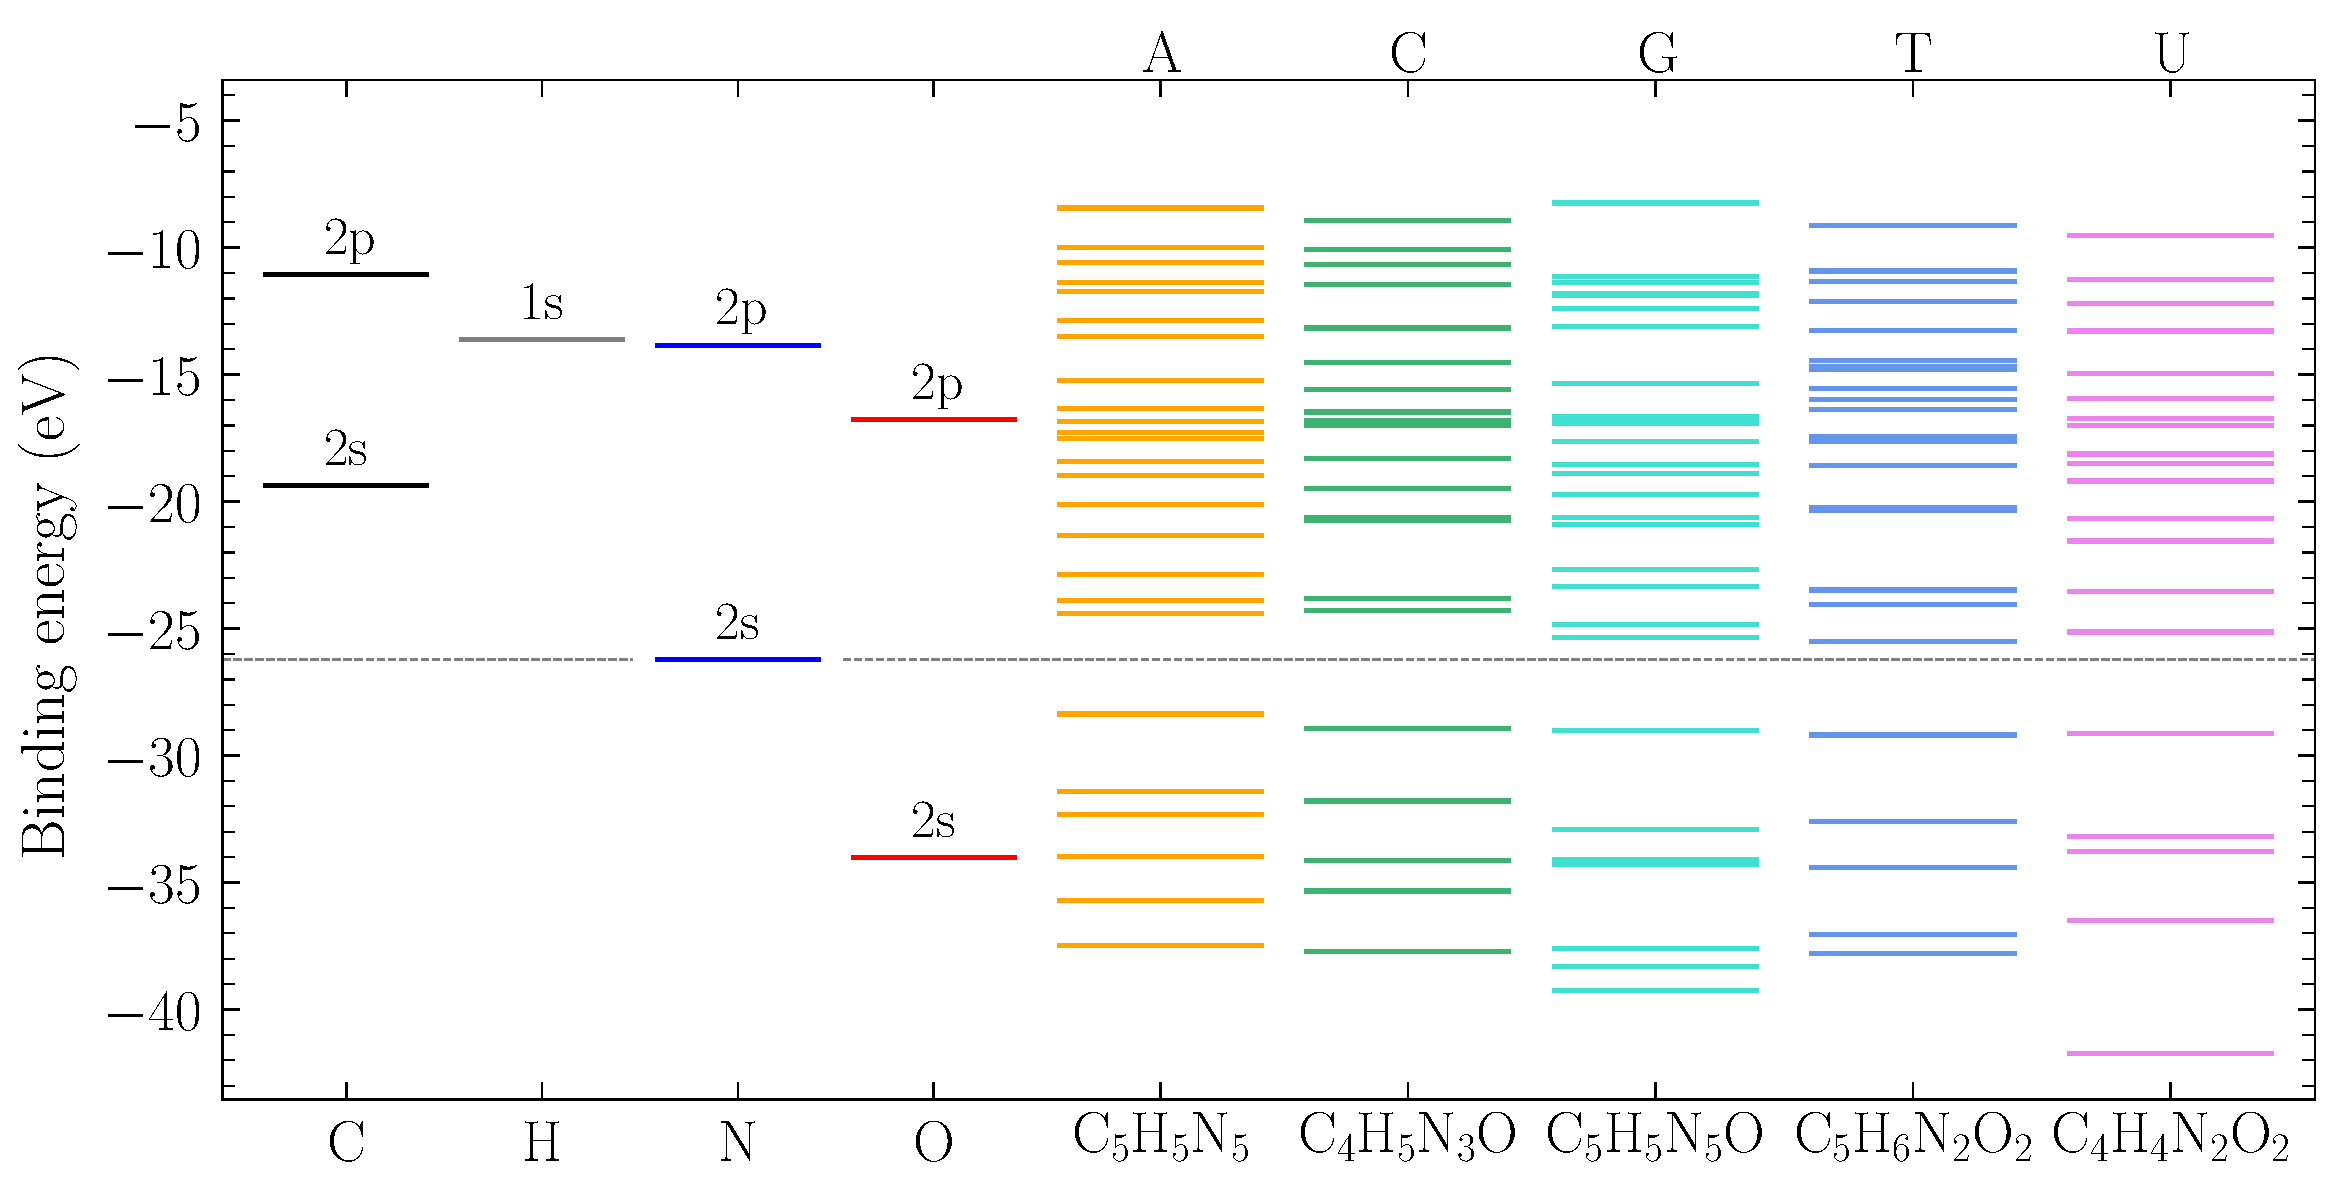
\includegraphics[width=0.9\textwidth]{ionmol/levelsDNA.eps}
\caption[Energías de ligadura moleculares teóricas de ADN y ARN.]
{Energías de ligadura moleculares teóricas de adenina, citosina, 
guanina, timina, y uracilo, comparado con los valores correspondientes 
de los átomos que las constituyen.}
\label{fig:ADNbindener}
\end{figure}

En la Fig.~\ref{fig:ADNbindener} se muestran las energías de ligadura 
molecular de los electrones de valencia para las nucleobases de ADN y 
uracilo. Las energías de ligadura del orbital molecular más alto (HOMO) 
que se obtienen concuerdan con los valores 
experimentales~\cite{Hush,Verkin,Dougherty} en un 2\% para todas las 
moléculas consideradas. En la izquierda de la Fig.~\ref{fig:ADNbindener}, 
se muestran las energías atómicas de Hartree-Fock de los elementos 
constituyentes. Esta comparación da una idea de la distribución de los 
electrones débilmente ligados en las moléculas. Se traza una línea 
discontinua alrededor de $-26$~eV para separar la banda molecular en 
dos. Los niveles de energía atómica por encima de esta línea se pueden 
considerar como los correspondientes a los electrones débilmente ligados 
de la Ec.~(\ref{eq:neCDW}). Por ejemplo, los electrones $2s$ y $2p$ del 
carbono se ubican por encima de la línea discontinua, que corresponde a 
los cuatro electrones dados por los números CDW. En el caso de oxígeno, 
solo los cuatro electrones de los orbitales 2p se encuentran por encima 
de la línea divisoria propuesta, que se corresponde con el número de 
electrones débilmente ligados dado por los valores CDW. El caso del 
átomo de nitrógeno no es tan directo; el número $\nu_{N}^{\text{CDW}}=4$ 
sugiere que sólo uno de los dos electrones de la capa $2s$ contribuye al 
esquema molecular.

%%%%%%%%%%%%%%%%%%%%%%%%%%%%%%%%%%%%%%%%%%%%%%%%%%%%%%%%%%%%%%%%%%%%%%%%
\subsection{Modelo estequiométrico modificado}
%%%%%%%%%%%%%%%%%%%%%%%%%%%%%%%%%%%%%%%%%%%%%%%%%%%%%%%%%%%%%%%%%%%%%%%%

El modelo estequiométrico propuesto en la Sección~\ref{sec:SSM} 
considera a la molécula $M$ como un conjunto de átomos neutros aislados, 
lo cual es completamente irreal. Una primera mejora al modelo se puede 
sugerir asumiendo que los átomos no son efectivamente neutros y que 
tienen una distribución electrónica dispar dentro de la molécula. Esta 
característica puede expresarse mediante una carga efectiva $q_{\alpha}$ 
por átomo. La carga de Mulliken proporciona un valor posible para 
$q_{\alpha}$; sin embargo, existe una gran variedad de posibles 
distribuciones de carga~\cite{lee2003}.

\begin{table}
\begin{center}
\begin{tabularx}{\textwidth}{
>{\centering\arraybackslash}p{0.15\textwidth}
>{\centering\arraybackslash}p{0.08\textwidth}
>{\centering\arraybackslash}p{0.08\textwidth}
>{\centering\arraybackslash}p{0.08\textwidth}
>{\centering\arraybackslash}p{0.08\textwidth}
>{\centering\arraybackslash}p{0.32\textwidth}}
\rowcolor{mydarkgray} 
Molécula & C & H & N & O & Estequiometría de carga \\
Adenina & $+0.32$ & $+0.23$ & $-0.55$ &       & 
C$_{4.92}$H$_{4.77}$N$_{5.14}$ \\ 
\rowcolor{mygray} 
Citosina & $+0.28$ & $4+0.21$ & $-0.56$ & $-0.53$ & 
C$_{3.93}$H$_{4.79}$N$_{3.14}$O$_{1.13}$ \\ 
Guanina & $+0.46$ & $+0.20$ & $-0.58$ & $-0.36$ & 
C$_{4.89}$H$_{4.80}$N$_{5.15}$O$_{1.09}$ \\ 
\rowcolor{mygray} 
Timina & $+0.20$ & $+0.19$ & $-0.54$ & $-0.52$ & 
C$_{4.95}$H$_{5.81}$N$_{2.13}$O$_{2.13}$ \\ 
Uracilo & $+0.31$ & $+0.22$ & $-0.59$ & $-0.47$ & 
C$_{3.92}$H$_{3.78}$N$_{2.15}$O$_{2.12}$ \\ 
\end{tabularx}
\caption[Cargas efectivas medias de Mulliken por átomo]
{Cargas efectivas medias de Mulliken por átomo $q_{\alpha}$, y nueva 
fórmula estequiométrica definida por la Ec.~(\ref{eq:newstoi}) para 
cinco moléculas de ADN.}
\label{tab:newstoi}
\end{center}
\end{table}

Para tomar en cuenta este efecto, se considera que el número total 
de electrones $Q_{\alpha }$ en el elemento $\alpha$ se distribuye de 
forma dispar sobre todos los átomos $\alpha$. Por lo tanto, cada 
elemento $\alpha$ tendrá una carga $q_{\alpha}=Q_{\alpha}/n_{\alpha}$ 
asociada, que puede ser positiva o negativa. Este valor dependerá de la 
electronegatividad relativa respecto a los otros 
átomos~\cite{rappe1991}. 
Siguiendo esta idea, se puede estimar el número fraccional de átomos por 
molécula $n_{\alpha}'$, el cual está dado por 
\begin{equation}
n_{\alpha }^{\prime }=n_{\alpha }-
\frac{q_{\alpha }}{\nu_{\alpha }^{\text{CDW}}}
\label{eq:newstoi}
\end{equation}
En el caso de átomos neutrales, $q_{\alpha}=0$ y 
$n_{\alpha}'=n_{\alpha}$, como dispone el SSM. En la 
Tabla~\ref{tab:newstoi}, se muestra un valor promedio de carga efectiva 
por átomo $q_{\alpha}$ para C, H, N, y O en las cinco nucleobases, que 
se obtienen a partir de los cálculos de estructura molecular descritos 
en la sección anterior.

Implementando la Ec.~(\ref{eq:newstoi}) es posible determinar una nueva 
fórmula estequiométrica de carga, que se muestra en la última columna de 
la Tabla~\ref{tab:newstoi}). Ahora, en vez de tener un número entero de 
átomos $n_{\alpha}$, se tiene un número fraccional dado por 
$n_{\alpha}'$. Considerando estos valores, se pueden calcular nuevas 
secciones eficaces moleculares, 
$\sigma'_{M}=\sum_{\alpha}n_{\alpha}'\sigma_{\alpha}$. Los errores 
relativos de las secciones eficaces de ionización con el SSM modificado 
para las bases de ADN de la Tabla~\ref{tab:newstoi} presentan 
diferencias menores al 3\% respecto a los valores previos. Esta 
comparación sugiere que el modelo estequiométrico es un modelo simple 
pero robusto, capaz de modelar este tipo de moléculas complejas dentro 
del margen de error esperado.

%%%%%%%%%%%%%%%%%%%%%%%%%%%%%%%%%%%%%%%%%%%%%%%%%%%%%%%%%%%%%%%%%%%%%%%%
\section{Conclusiones}
%%%%%%%%%%%%%%%%%%%%%%%%%%%%%%%%%%%%%%%%%%%%%%%%%%%%%%%%%%%%%%%%%%%%%%%%

En este Capítulo, se estudió la ionización de blancos moleculares de 
interés biológico debido al impacto de iones de carga múltiple. La 
aproximación teórica propuesta combina el modelo estequiométrico simple, 
para describir la molécula, y el método de onda distorsionada con estado 
inicial de Eikonal para blancos atómicos (descritos con potenciales 
DIM), para modelar el proceso colisional. Se calcularon secciones 
eficaces de ionización de un gran número de blancos moleculares de 
interés biológico conteniendo H, C, N y O por el impacto de 
antiprotones, H$^{+}$, He$^{2+}$, Be$^{4+}$, C$^{6+}$, y O$^{8+}$. 
En particular, se examinaron las secciones eficaces de ionización total 
simple de adenina, citosina, timina, guanina, uracilo, THF y agua, 
siendo éstas comparadas a su vez con datos experimentales disponibles. 

Se calcularon y estudiaron valores medios de energía y ángulo de emisión 
de los electrones eyectados de blancos atómicos, que son de importancia 
en el daño secundario de las colisiones con iones. Los resultados CDW
muestran una clara dependencia de estos valores con la carga del ion 
$Z$. Para un blanco dado, a medida que $Z$ aumenta, los valores de
$\overline{E}_{\alpha}$ también aumentan. Por otro lado, las 
predicciones de $\overline{\theta}_{\alpha}$ decrecen, lo que muestra 
una clara tendencia de eyección en la dirección del ion. A energías de 
impacto mayores a 2~MeV/amu, estos valores convergen a la primera 
aproximación de Born, la cual establece la simple ley de escala $Z^{2}$. 

Se propusieron tres reglas de escala para las secciones eficaces de 
ionización en blancos de interés biológico por cuatro iones desnudos. 
Primero, se exploró la ampliamente usada regla de escala de Toburen, que 
escala la sección eficaz de ionización molecular con un determinado 
número de electrones débilmente ligados. Luego, a partir de los 
resultados CDW para los atómos H, C, N y O, se encontró que la respuesta 
de las secciones eficaces de ionización puede ser optimizada 
normalizándolas con diferentes números de electrones activos en la 
colisión. Así, la primera regla de escala reduce las secciones eficaces 
moleculares con el número de electrones activos CDW, la cual provee 
buenos resultados para los sistemas proyectil--molécula estudiados aquí. 
La comparación con los datos experimentales refuerza la primera ley de 
escala propuesta. La regla de escala con números CDW se probó incluyendo 
datos experimentales de ionización de H$_2$, metano y amoníaco por 
impacto de protones, los cuales mostraron una buena concordancia en el 
rango de energías intermedias a altas. La segunda regla de escala 
consideró la naturaleza del proyectil; así, la sección eficaz de 
ionización se reduce con la carga del ion incidente, $Z^{\alpha}$, como 
una función de la energía incidente reducida $E/Z^{2-\alpha}$, siendo 
$\alpha=1.2$. La última ley de escala se obtuvo de la conjunción de las 
dos primeras: la sección eficaz de ionización total se reduce con el 
número de electrones activos CDW y la carga del ion, $Z^{\alpha}$. Esta 
combinación conduce a una ley de escala de tipo universal, independiente 
de la carga del ion y el blanco molecular. Se compararon las tres reglas 
de escala obtenidas mediante el modelo SSM--CDW para los 80 sistemas 
colisionales examinados con datos experimentales disponibles. 
Finalmente, se probó la generalidad de la regla de escala independiente 
mediante la inspección de un número significativo de datos 
experimentales para sistemas colisionales ajenos a este trabajo. Se 
encontró que la regla de escala universal propuesta es válida incluso 
para energías fuera del rango de validez del método SSM--CDW.

También se realizaron cálculos de estructura molecular para las 
nucleobases del ADN. Al inspeccionar las energías de ligadura 
moleculares obtenidas mediante cálculos cuánticos de primeros principios, 
se pudo comprender el número de electrones activos resultantes de la 
optimización basada en los cálculos CDW. Se propuso un modelo 
estequiométrico modificado utilizando la carga de Mulliken para obtener 
proporciones fraccionarias en lugar de enteras para el número de átomos 
constituyentes. No se encontró una corrección sustancial, lo que indica 
que el SSM tiene un buen desempeño. El extenso análisis de los 
resultados presentados refuerzan la validez del modelo estequiométrico 
simple en combinación con la aproximación CDW para tratar la ionización 
de moléculas complejas por el impacto de iones de carga múltiple en el 
rango de energía intermedia a alta. 


